%!TEX root = ../main

\section{Tensor Parallelism NLP}

Следующий текст отражает \cite{shoeybi2019megatron}.

У нас есть классные задачки на NLP, модели GPT-2 и Bert, которые достигли State-of-the-art (выдающихся результатов) в решении каких-то сложных задач. Но есть проблема - они состоят из большого количества параметров и требуют довольно много данных чтобы обучится. В итоге обучить их становится довольно трудно, если использовать только один процессор.

Поэтому люди делают обучение многопоточным. Некоторые популярные способы: 
\begin{enumerate}
    \item Разбивают данные на партии (batch-и), и их отдают модели параллельно на несколько GPU. Затем результаты агрегируются через функцию (например берется среднее градиентов для последующего изменения весов модели)
    \item  Делают модель распределенной. Разбивают модель на набор операций, и разносят их по процессам, а затем синхронизируют. Здесь нужна дополнительная логика поверх используемой модели. 
\end{enumerate}
Авторы используют немного другой подход. Одни из самых частых операций - это вычисления с тензорами (например перемножения матриц). Поэтому можно разбить тензор параметров модели на несколько, все полученные составляющие раскидать по разным GPU, каждому отдать одни и те же входные данные, и запустить параллельную обработку. Если в модели есть нелинейный слой, требующий всех данных сразу - собрать результат с всех процессоров и пропустить через нее. Чем меньше точек синхронизации, тем лучше производительность. А из-за того, что мы разбиваем элементы модели, не меняя особо процесс ее обучения - то изменения нужны минимальные.

Описанные дальше подходы можно применять для любой подходящей модели, но авторы взяли задачи NLP. В основе наиболее успешных моделей лежат трансформеры (Transformers). Его истоки состояли из RNN - что вообще не ложится на параллельность. Но \cite{vaswani2017attention} от реккурентости избавляются, что позволяет обрабатывать входные данные и выполнять некоторые слои параллельно. Теперь трансформеры - корень всех моделей, их можно разбить на encoder-а и decoder-а, собирать их последовательно, навешивать дополнительные слои, обучать модели для разных задач и получать удивительные результаты. Bert обучался понимать структуру языка, изначально решая набор базовых задач (как вставить правильное слово в пропуск и сказать про предложения - они связаны или нет). Затем он дообучается для более конкретной задачи. GPT-2 это модель которая умеет по началу предложения генерировать продолжение. Сначала GPT уступало Bert, но разработчики значительно увеличили количество параметров до 1.5 млдр, сделав ее самой большой на тот момент, разнообразили датасет из статей из интернета, и она достигла воистину state-of-the-art, ее даже боялись публиковать полностью. Поэтому чтобы ускорить модели, можно оптимизировать именно трансформеры.

 Это модель трансформера, взятая авторами статьи:
 

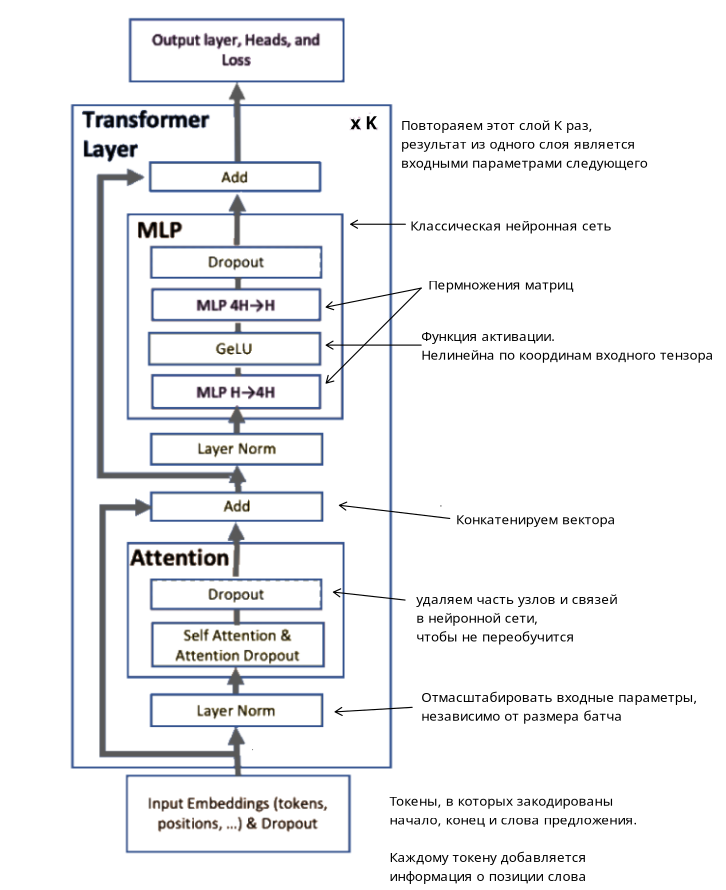
\includegraphics[width=0.6\linewidth]{Parts/images/TP_Transformer.png}

Найдем, где в этой модели используется перемножение матриц. В более простом блоке нашей модели - MLP преобразования будут следующими:

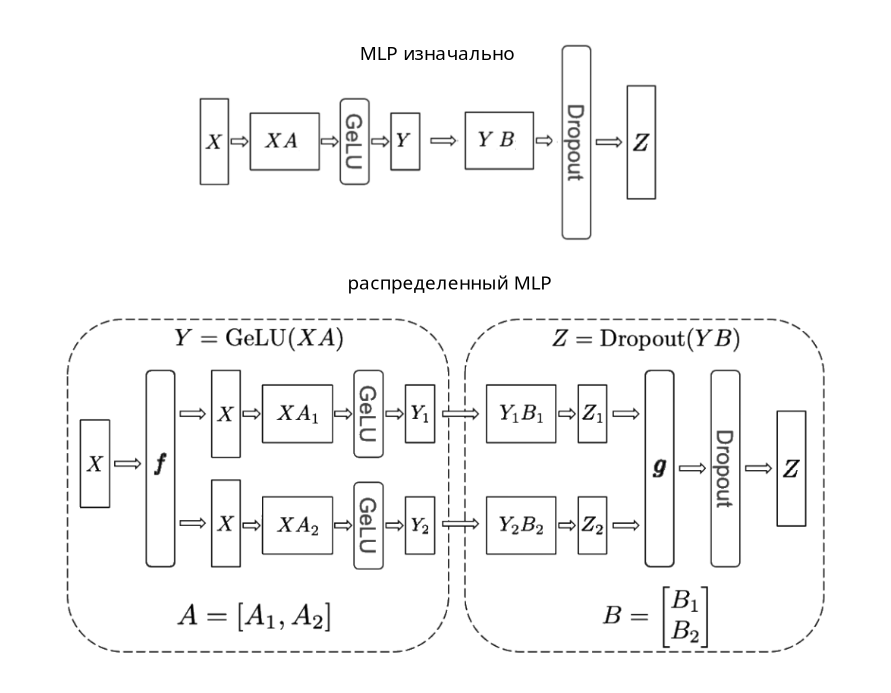
\includegraphics[width=0.6\linewidth]{Parts/images/TP_MLP.png}

Если посмотреть на них внимательно, то обе схемы почти одинаковые. Только в нижней есть блок f, который в прямом проходе дублирует данные на несколько GPU, и блок g - который собирает данные с нескольких процессоров в одну матрицу. Эти блоки являются точками синхронизации, и их на каждый проход (прямой и обратный для релаксации весов) по 2 для одного Transformer Layer-а. 


Аналогично поступаем и для слоя внимания

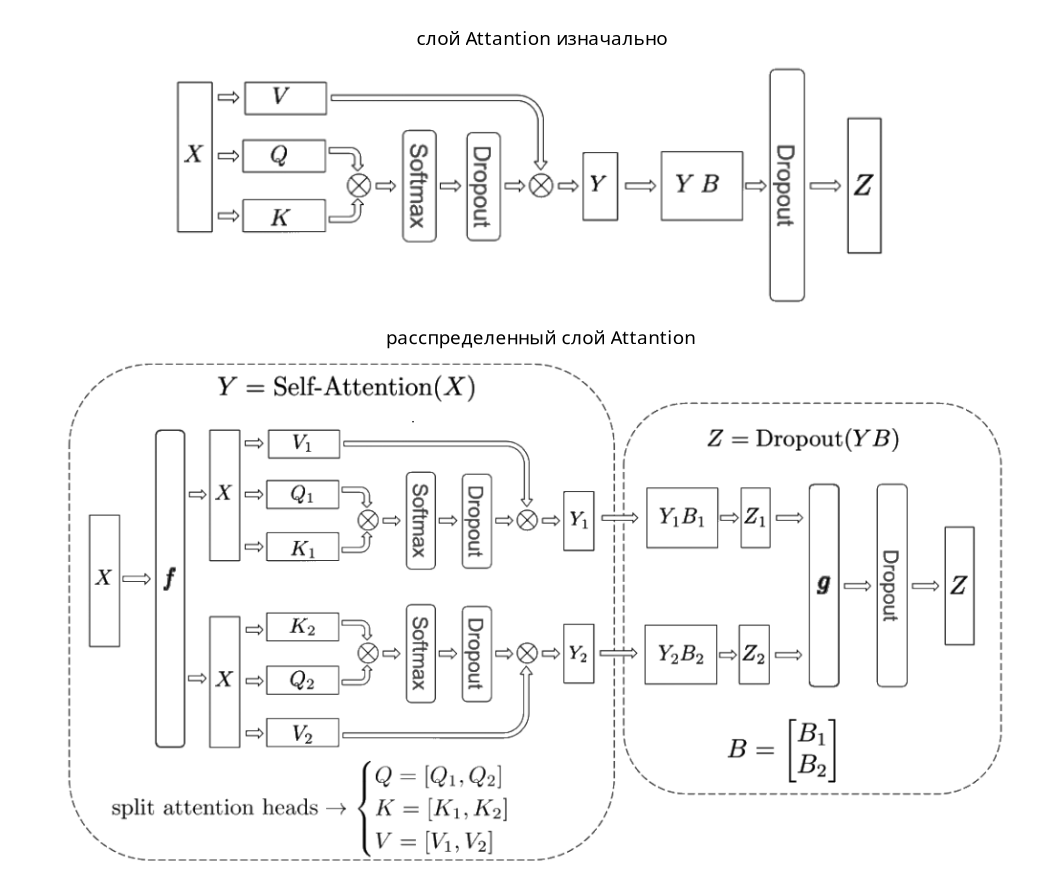
\includegraphics[width=0.6\linewidth]{Parts/images/TP_Attention.png}

Получаем распараллеленную модель, добавив всего два простых блока f и g.


Некоторые модели могут отличаться от представленного в статье, но почти любое перемножение матрица можно параллелить, не забывая потом добавлять простой объединяющий слой когда нужно. 

Еще одно  улучшение - перед тем, как считать cross entropy, мы должны отправить одному процессору объединенную матрицу. Одной из ее размерностью является размер словаря, что для хороших моделей будет большой. Там будут находится вероятности для данного слова быть в предложении следующим. Так вот, всю эту размерность можно схлопнуть, если считать  cross entropy на каждом GPU работающем параллельно, и отправлять уже меньше данных. Авторы говорят, что это сильно улучшило их время обучения. 

Теперь интересно посмотреть на то, как хорошо это работает.

Для обучения моделей был собран единый датасет из существующих (тексты с Википедии, новостей и тд), который весил 174 Гибибайтов. 

Сначала применили паралелизацию описанную выше для 1-2-48 GPU, и посмотрели на эффективность (на графике синие столбца). Раньше я также говорила про один из способов ускорить обучение - разбить данные на batch-и. Это называется data parallel, и его можно также внедрить в схему. До этого мы обучающие данные копировали полностью на несколько GPU, и на каждом работали с разными весами модели. Теперь можно вместо одной GPU в схеме, поставить 64 идентичных, полностью скопировать внутреннее состояние, а вот входные данные разбить между ними. Получается что так мы сначала делим модель, а затем входные embedding-и. Используемых GPU получаем больше, измеряем эффективность распределенных вычислений на них и рисуем зеленные столбцы.

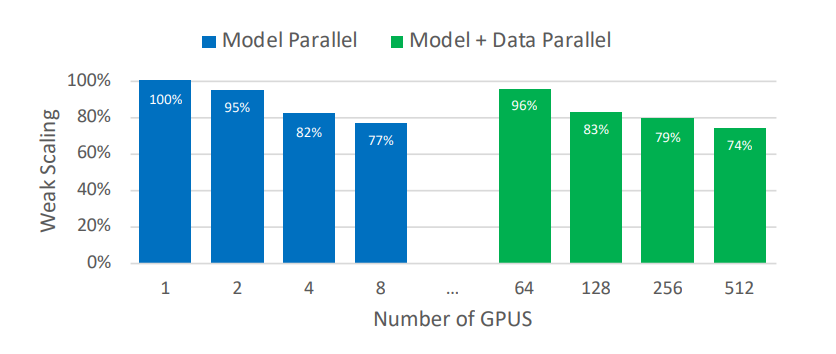
\includegraphics[width=0.8\linewidth]{Parts/images/TP_weak_scaling.png}

Что вообще на этом графике изображено и про что weak scaling? Для его измерения мы увеличиваем количество GPU и количество входных данных нашего датасета для нашей модели. В идеальном мире, время работы каждого отдельного процессора не должно изменится, ведь он обрабатывает одно и тоже количество данных, и это мы называем 100\%. Но в реальном мире у нас есть накладки например в виде времени обмена данными между GPU, и поэтому время работы немного увеличивает по сравнению с идеальным вариантом. Weak Scaling здесь показывает эффективность наших действий с добавлением большего числа GPU по сравнению с идеальным вариантом.

В итоге, авторы статьи достигают 77\% и 74\% по сравнению с наилучшим вариантом, в котором бы при увеличении размера входных данных время обучения бы не изменилось. Чтобы как-то ощутить сколько это хорошо, модель GPT-2 которая имеет 355 миллиона параметров обучалась одну эпоху за 20.6 часов, а модель с 8.3 миллиардами (в 23 раза больше) - за 50.4 часов, что является самой большой моделью, что когда-либо собирали на момент написания статьи.

Более того, большие модели показывают лучше результат - на графиках видно, что чем больше параметров у модели, тем меньше функции потерь. На втором графике архитектура (a) (классический Bert) от архитектуры (b) (на что мы смотрели в этой статье) отличается количеством вектором, проходящих через слов Layer Norm. Как видно на графике, у классического Bert-а с большим числом параметров начинает переобучение, поэтому авторам статьи пришлось изменить модель.  

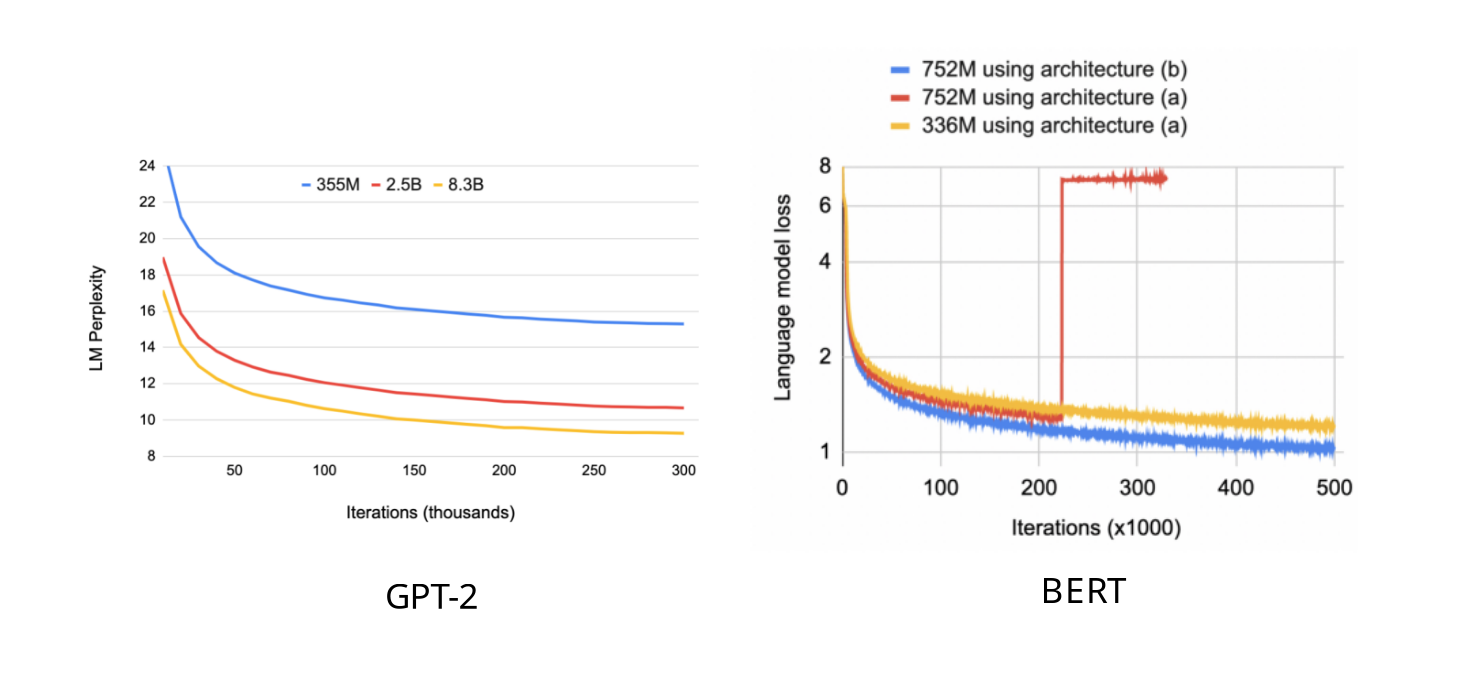
\includegraphics[width=0.8\linewidth]{Parts/images/TP_loss.png}

Суммируя рассказ, модели нейронных сетей с большим количеством параметров могут работать лучше, но также требуют значительно больше временных ресурсов чтобы обучится. Можно использовать больше процессоров, и внеся довольно мало изменений в работу программ, в итоге получить результаты за более разумное время.
